\chapter{Arquitectura hardware del sistema}
\label{cap:capitulo5}

\begin{flushright}
\begin{minipage}[]{10cm}
\emph{Las grandes cosas se hacen por una serie de pequeñas cosas reunidas juntas.}\\
\end{minipage}\\

Vincent van Gogh\\
\end{flushright}

\vspace{1cm}

Una vez presentadas las plataformas de desarrollo utilizadas, este capítulo describe la arquitectura \textit{hardware} del sistema desarrollado.


\section{Diseño del robot}
\label{sec:hardware}

Para el diseño de la forma física del robot se tomaron como referencia diversos robots asistenciales ya existentes. La mayoría de ellos presentan una arquitectura similar, compuesta por una pantalla táctil para la interacción con el usuario, una pantalla adicional destinada a la representación de expresiones faciales y una base móvil con ruedas.

\vspace{0.2cm}

Entre los sistemas analizados destacan JUNO, un robot asistencial orientado a la prevención de caídas en personas mayores (Figura \ref{fig:asistencial} izda), y TEMI\footnote{https://intecrobots.com/producto/temi-robot-asistente-personal-recepcion/?srsltid=AfmBOoqfjMJItp1psGnledndvFqIcn8kBztA7HvcE6iInBlifHYQFKKc}, un robot asistente personal (Figura \ref{fig:asistencial} dcha).

\vspace{0.2cm}


\begin{figure}[H]
    \begin{center}
      \subcapcentertrue
      \subfigure[Robot JUNO]{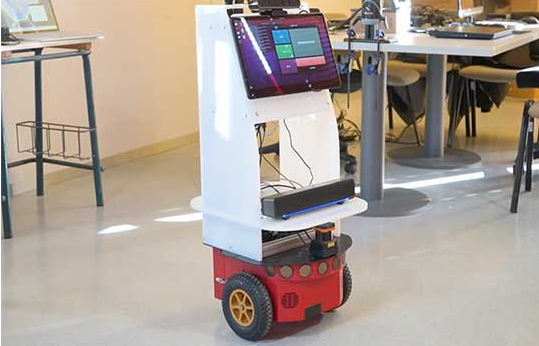
\includegraphics[width=64mm]{figs/juno}}
      \hspace{3mm}
      \subfigure[Robot TEMI de intect robots]{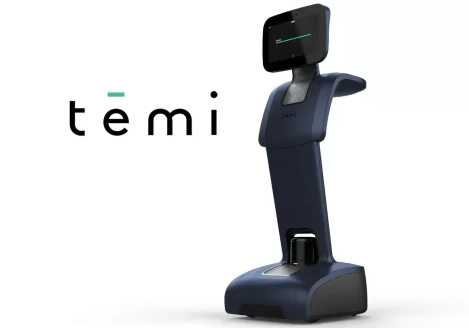
\includegraphics[width=65mm]{figs/temi}}
    \end{center}
    \caption{Robots asistenciales}
    \label{fig:asistencial}
  \end{figure}


\vspace{0.2cm}

En el diseño se consideraron aspectos relacionados con el ensamblaje y el mantenimiento del sistema, de forma que los distintos módulos se pudieran desmontar fácilmente para su reparación.

\vspace{0.2cm}

Se buscó garantizar la estabilidad del robot, por lo cual se optó por una configuración de tres ruedas en una disposición conocida como \textit{castor wheeled mobile robot}\footnote{https://robotechvision.com/caster/} como se muestra en la Figura \ref{fig:castor}, donde los puntos de apoyo forman un triángulo equilátero. Esta geometría maximiza el polígono de sustentación del sistema, asegurando que el centro de masas se mantenga de manera óptima dentro de los límites de soporte en condiciones operativas estándar, un principio fundamental en el análisis de estabilidad de robots móviles con ruedas \cite{pr11123302}.


\vspace{0.2cm}

\begin{figure} [h!]
  \begin{center}
    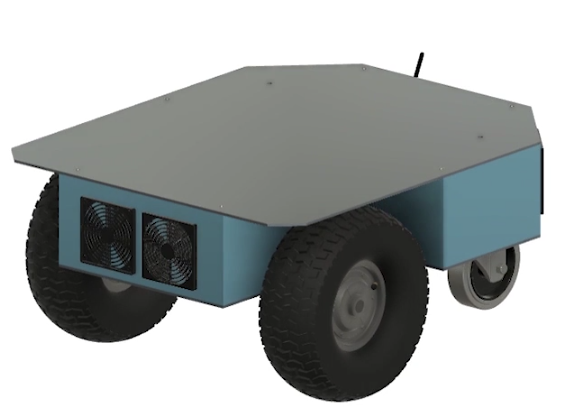
\includegraphics[width=9cm]{figs/castor}
  \end{center}
  \caption{Robot Caster de ROBO TECH}
  \label{fig:castor}
\end{figure}\


A partir de estas referencias se elaboraron una serie de bocetos iniciales (Figura \ref{fig:boceto}) con el objetivo de explorar distintas alternativas de diseño. Estos bocetos sirvieron como punto de partida para el proceso de prototipado.

\vspace{0.2cm}

\begin{figure} [h!]
  \begin{center}
    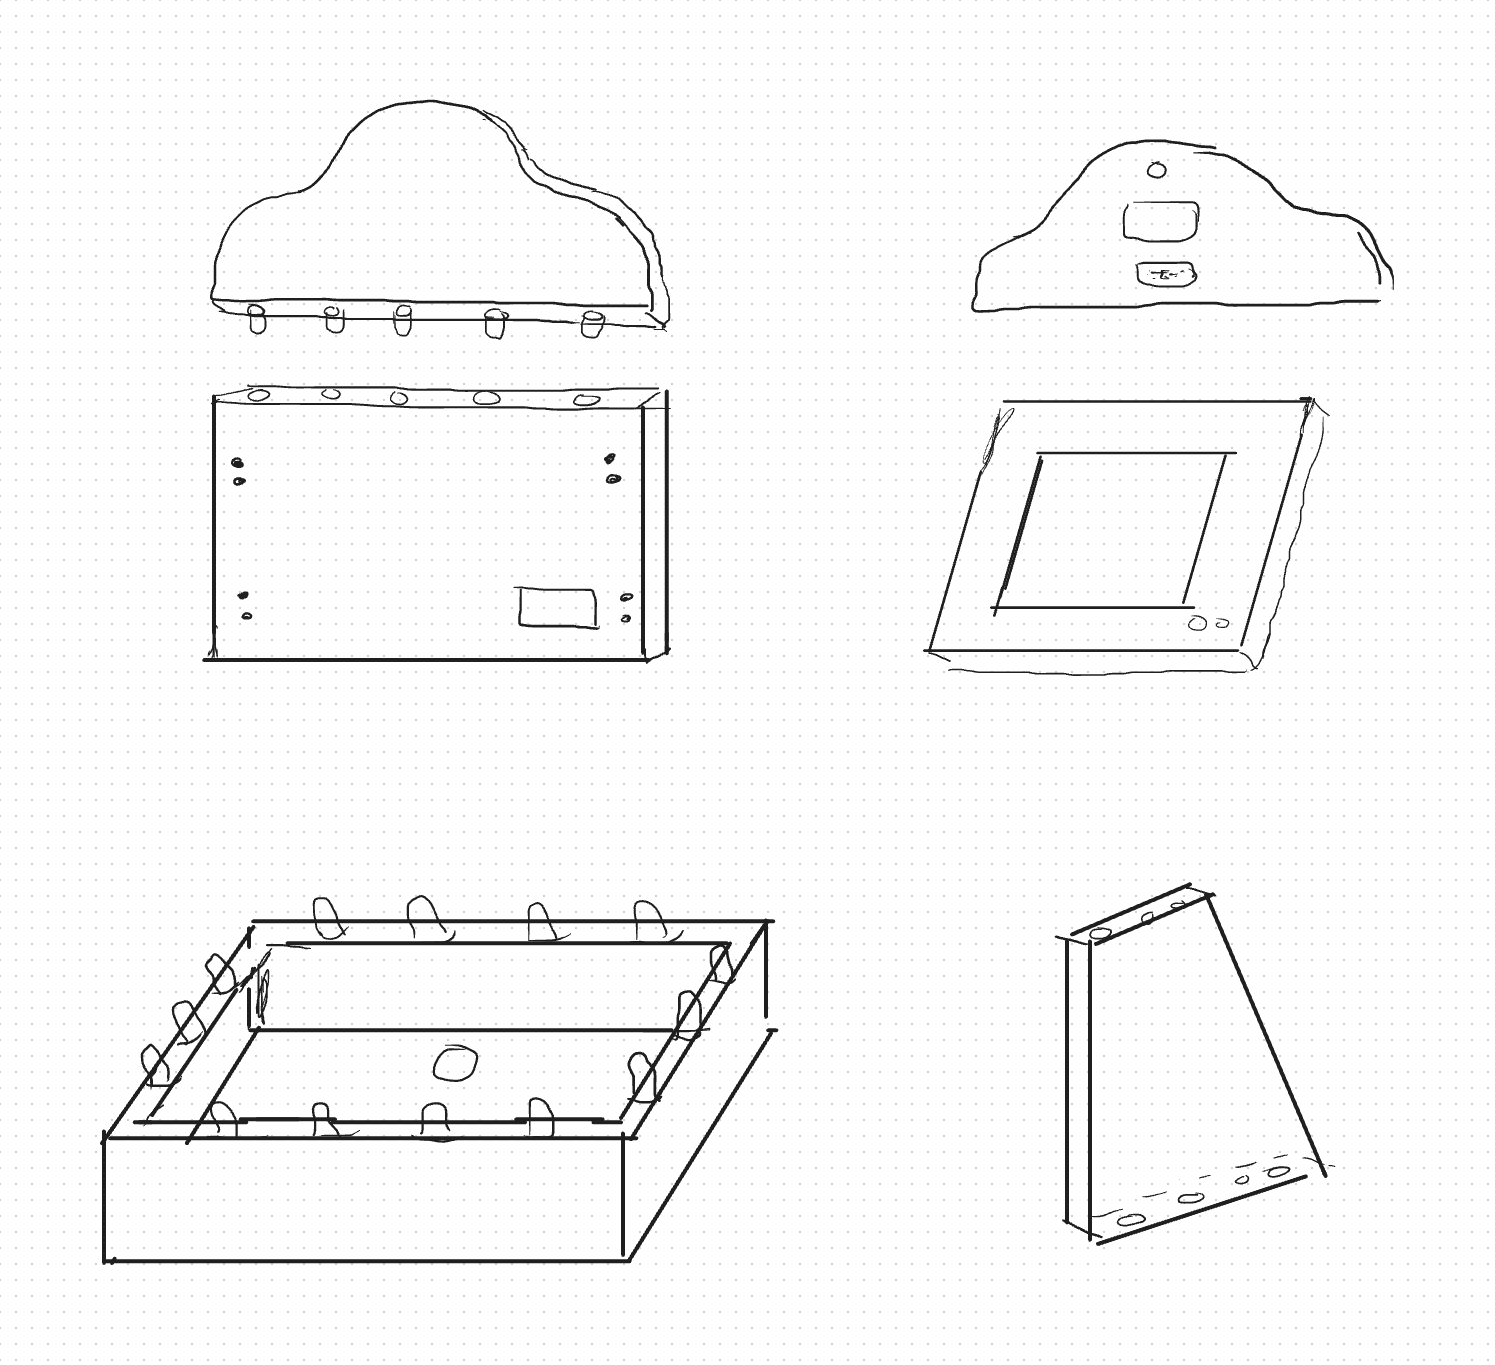
\includegraphics[width=14cm]{figs/boceto}
  \end{center}
  \caption{Boceto vistas}
  \label{fig:boceto}
\end{figure}\



\vspace{0.2cm}

Con el diseño preliminar definido, se construyó un prototipo físico utilizando cartón con el objetivo de validar las dimensiones generales del robot y analizar la disposición de los diferentes elementos. Esta fase permitió identificar posibles problemas de  diseño como la distribución de componentes, el espacio disponible y las dimensiones seleccionadas. Asimismo, permitió evaluar el volumen total del robot y su adecuación para operar en entornos reales.
En la Figura \ref{fig:modelo} se muestra el prototipado en cartón.

\vspace{0.2cm}


\begin{figure}[H]
  \begin{center}
    \subcapcentertrue
    \subfigure[Modelo del robot a cartón]{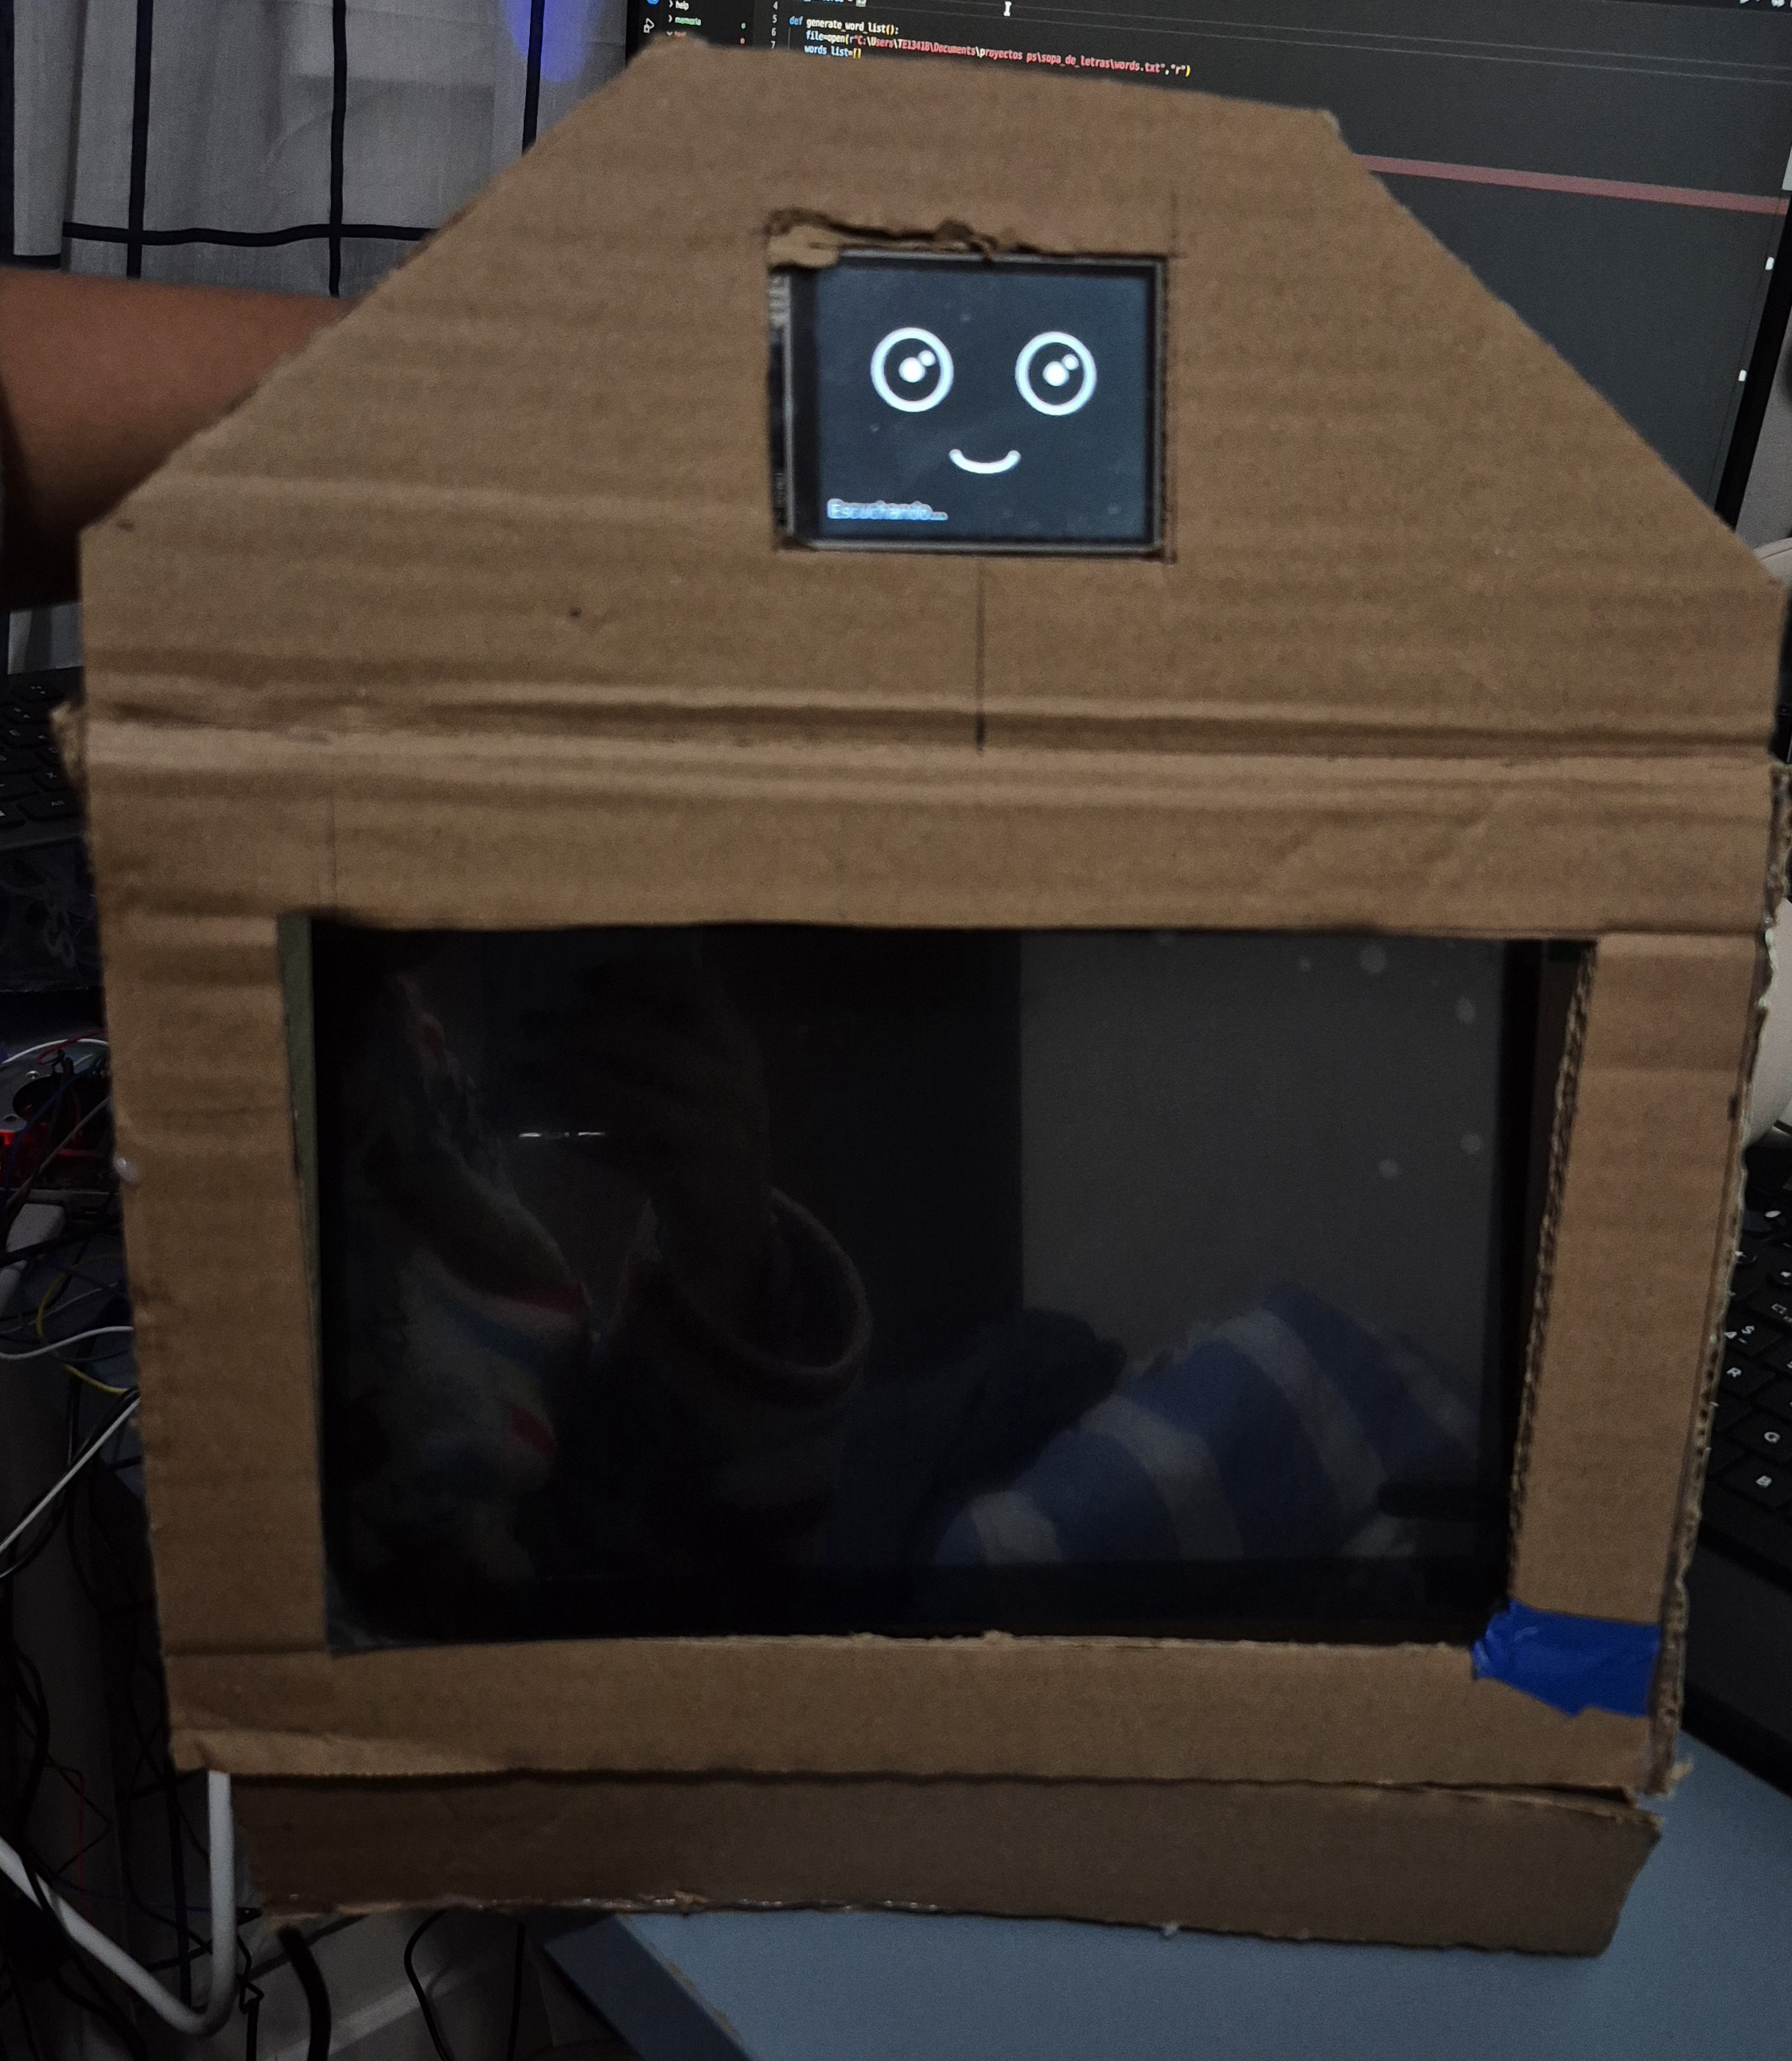
\includegraphics[width=0.48\textwidth, height=56mm, keepaspectratio=false]{figs/modelo_carton}}
    \hspace{3mm}
    \subfigure[Pieza de cartón base]{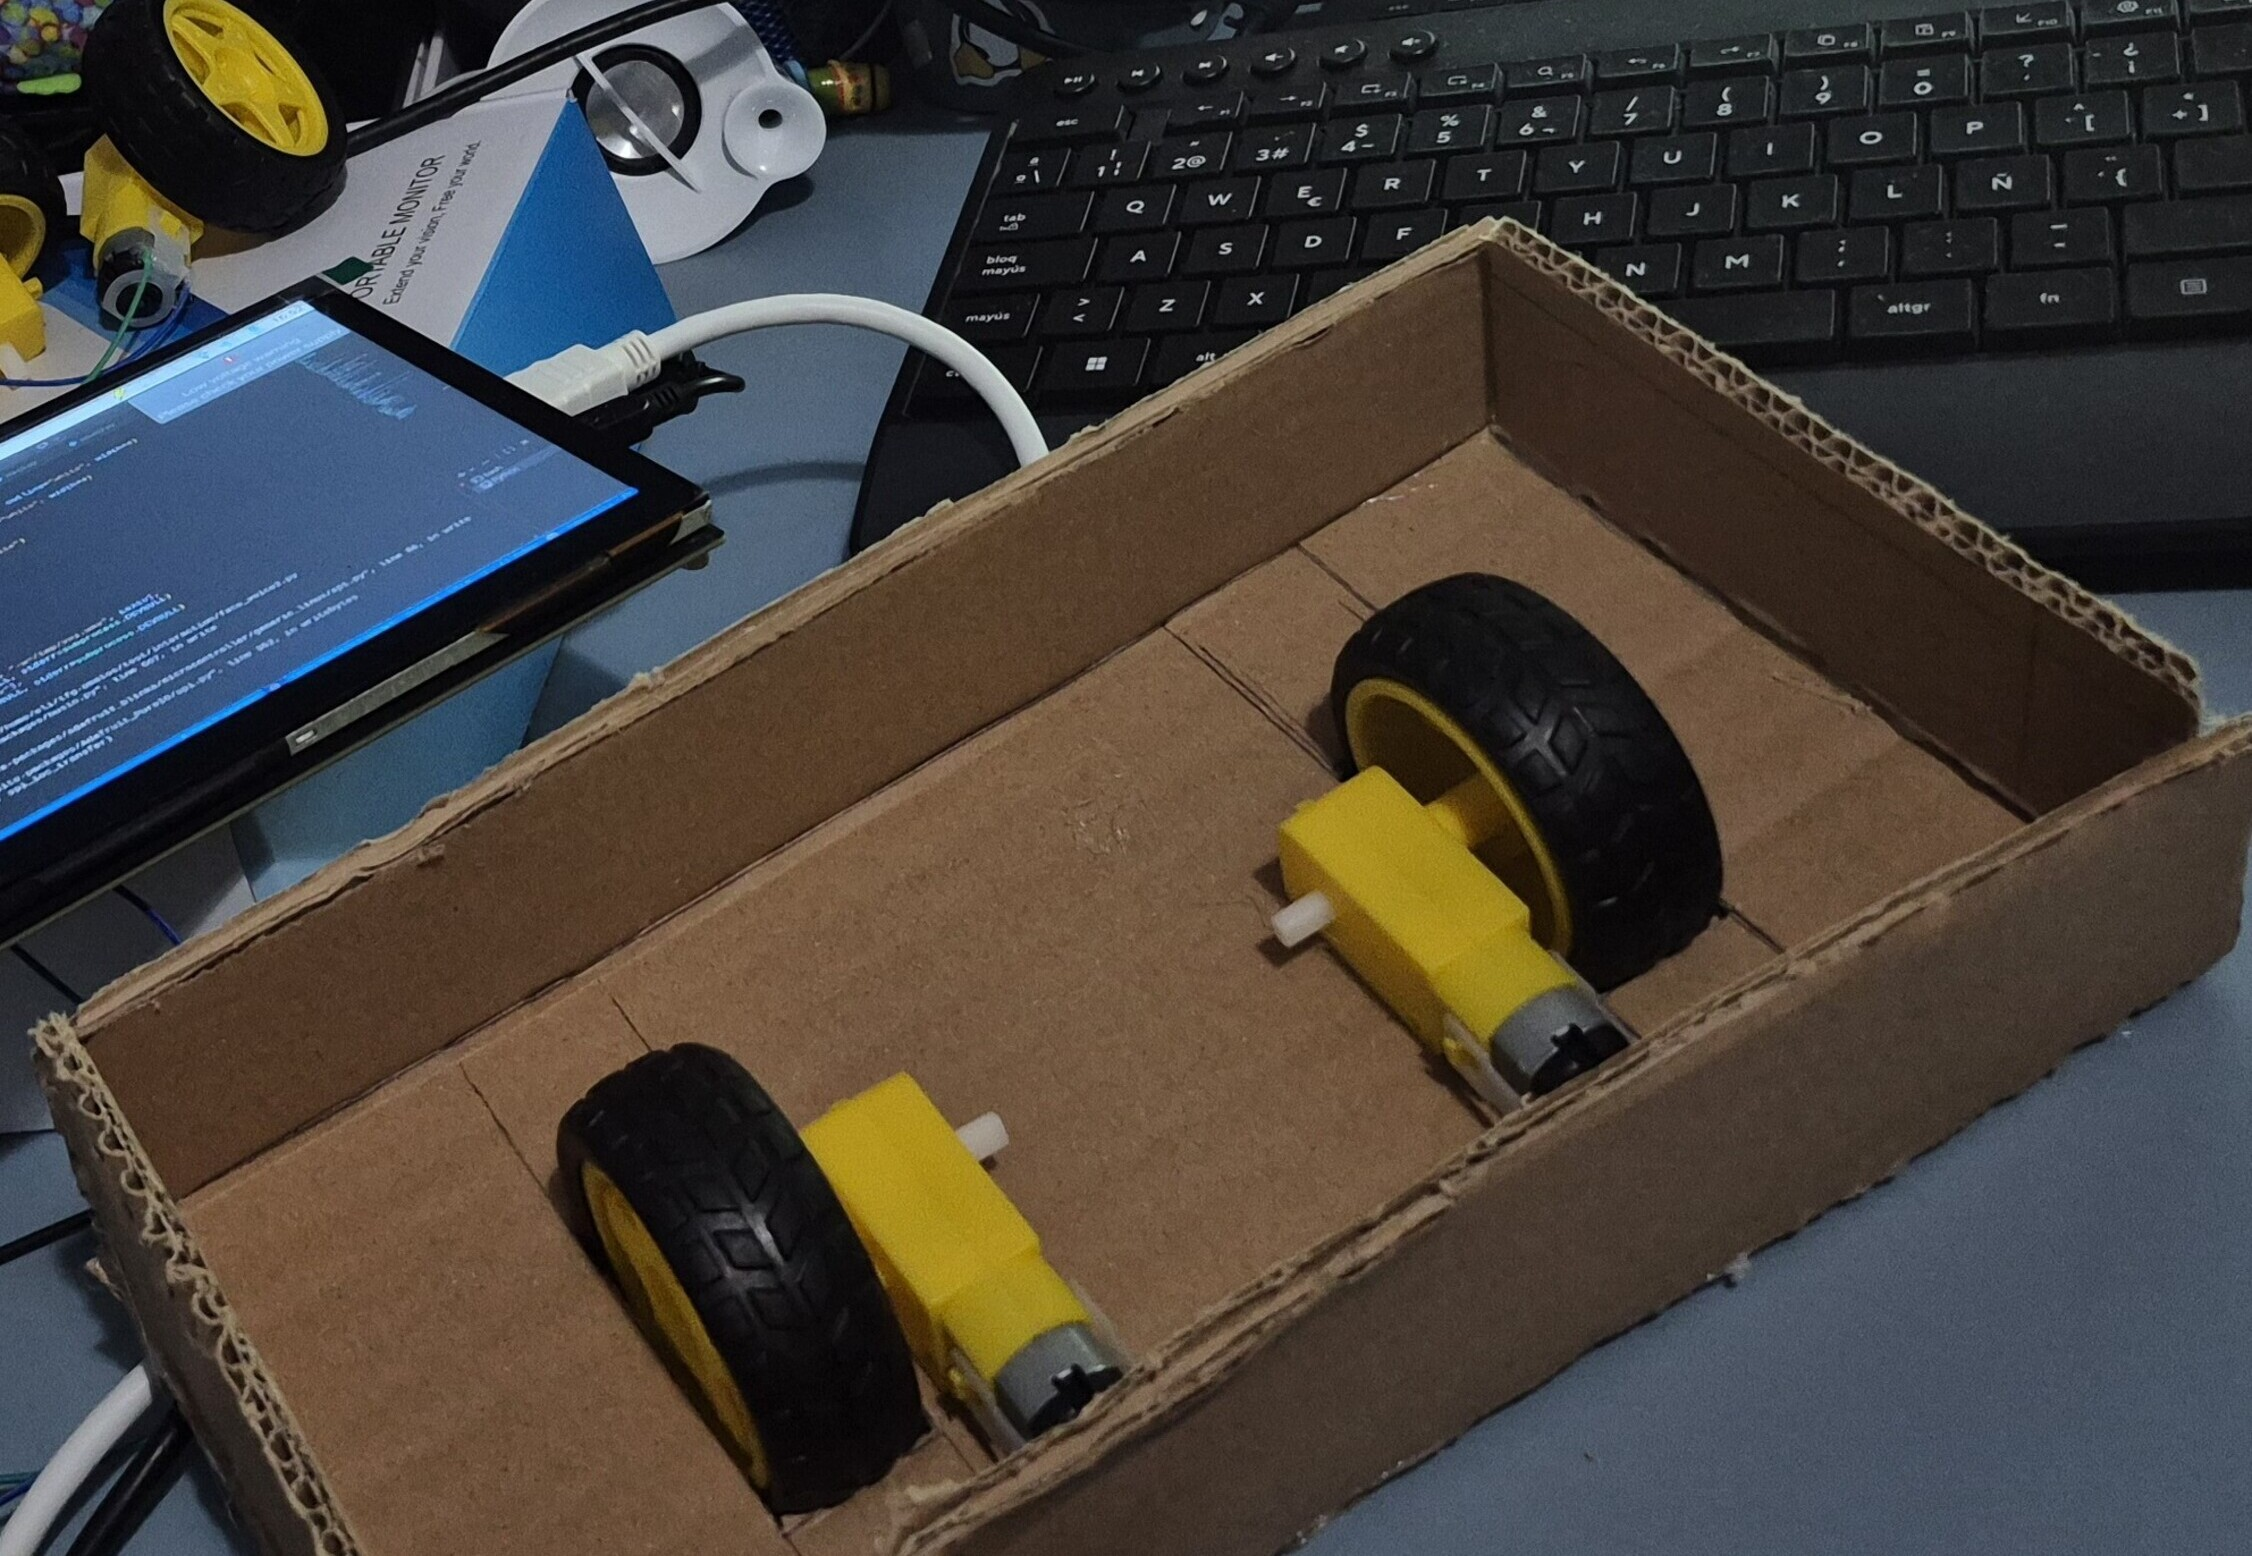
\includegraphics[width=0.48\textwidth, height=56mm, keepaspectratio=false]{figs/ruedas_carton}}
  \end{center}
  \caption{Prototipo a cartón}
  \label{fig:modelo}
\end{figure}


Una vez validado el diseño preliminar mediante el prototipo de cartón, se procedió al desarrollo del modelo tridimensional del robot utilizando el software libre FreeCAD. Este modelo permitió definir con mayor precisión la geometría de la estructura, ajustar las dimensiones y verificar la integración de los componentes que conforman el sistema dentro del espacio disponible.

Las Figuras \ref{fig:3D}, \ref{fig:3D1} y \ref{fig:3D2} muestran diferentes vistas del modelo tridimensional.

\vspace{0.2cm}

\begin{figure} [h!]
  \begin{center}
    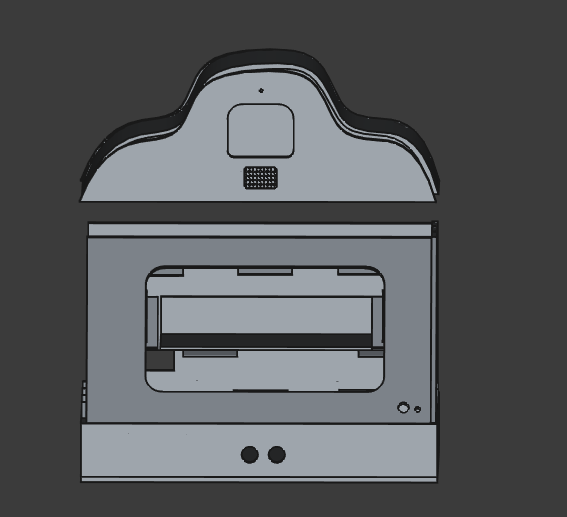
\includegraphics[width=10cm]{figs/3D2}
  \end{center}
  \caption{Vista frontal del modelo 3D en FreeCAD}
  \label{fig:3D2}
\end{figure}\


\begin{figure} [h!]
  \begin{center}
    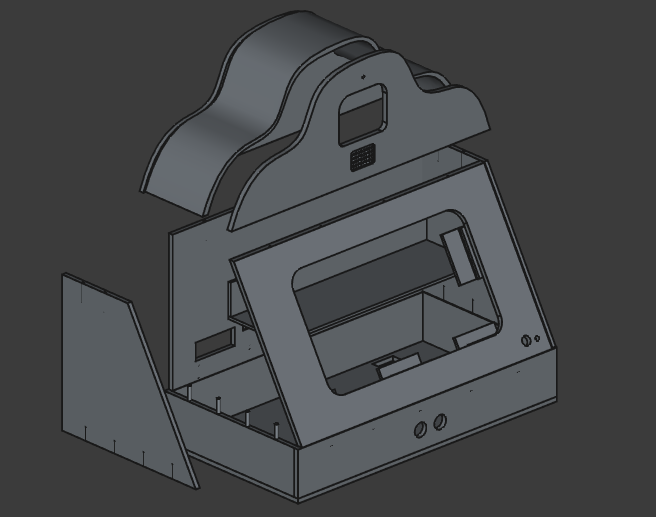
\includegraphics[width=10cm]{figs/3D}
  \end{center}
  \caption{Vista lateral del modelo 3D en FreeCAD}
  \label{fig:3D1}
\end{figure}\


\begin{figure} [h!]
  \begin{center}
    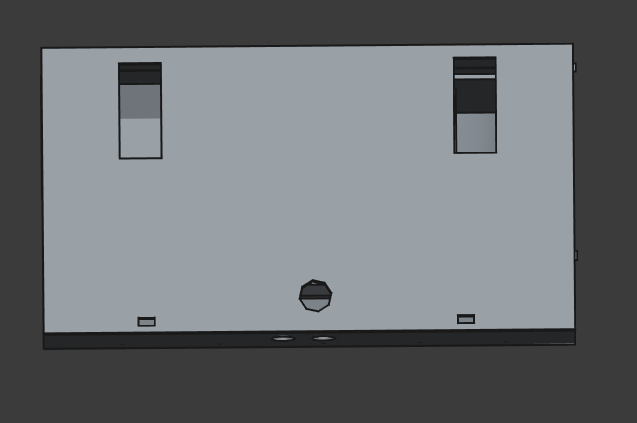
\includegraphics[width=10cm]{figs/3D3}
  \end{center}
  \caption{Vista inferior del modelo 3D en FreeCAD}
  \label{fig:3D}
\end{figure}\

Finalmente, a partir del modelo tridimensional desarrollado, se construyó la versión física del robot mediante piezas impresas en 3D de PLA (Ácido Poliláctico).

El resultado final del robot se muestra en la Figura \ref{fig:robot}, donde se presentan la estructura sin componentes electrónicos y el sistema completo montado.

\vspace{0.2cm}

\begin{figure}[H]
  \begin{center}
    \subcapcentertrue
    \subfigure[Estructura robot]{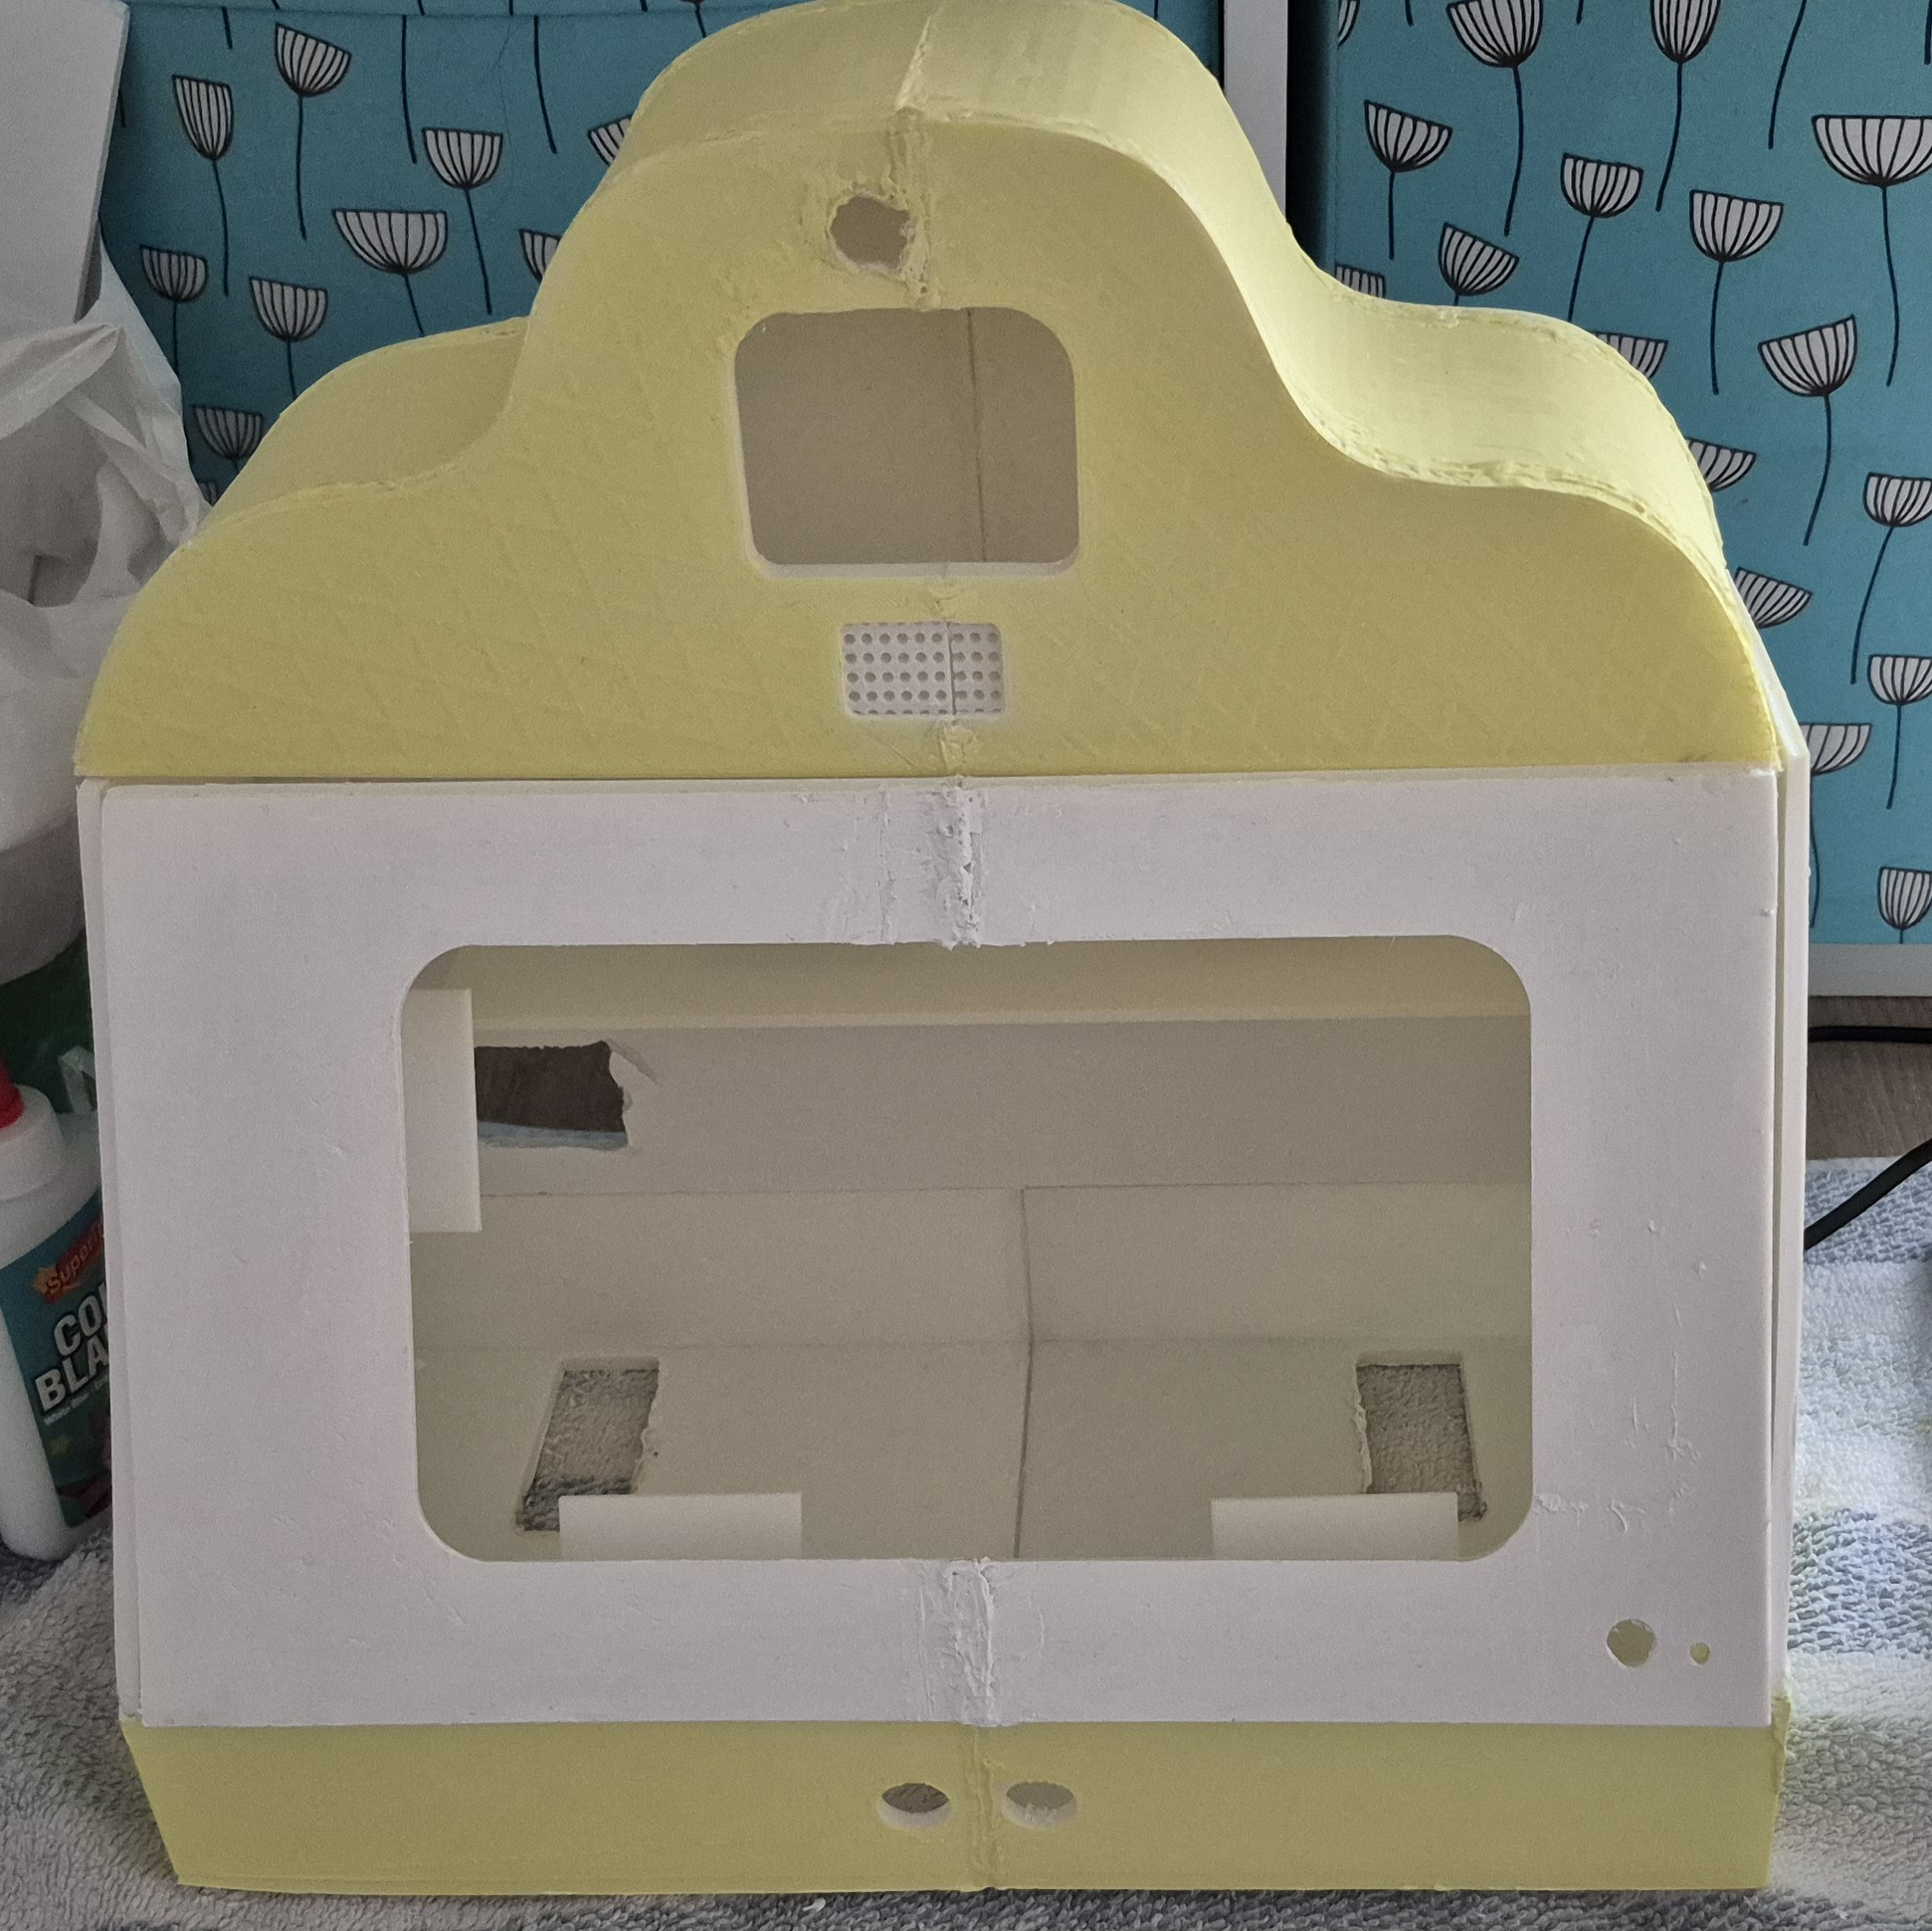
\includegraphics[width=0.48\textwidth, height=60mm, keepaspectratio=false]{figs/estructura1}}
    \hspace{3mm}
    \subfigure[Sistema completo]{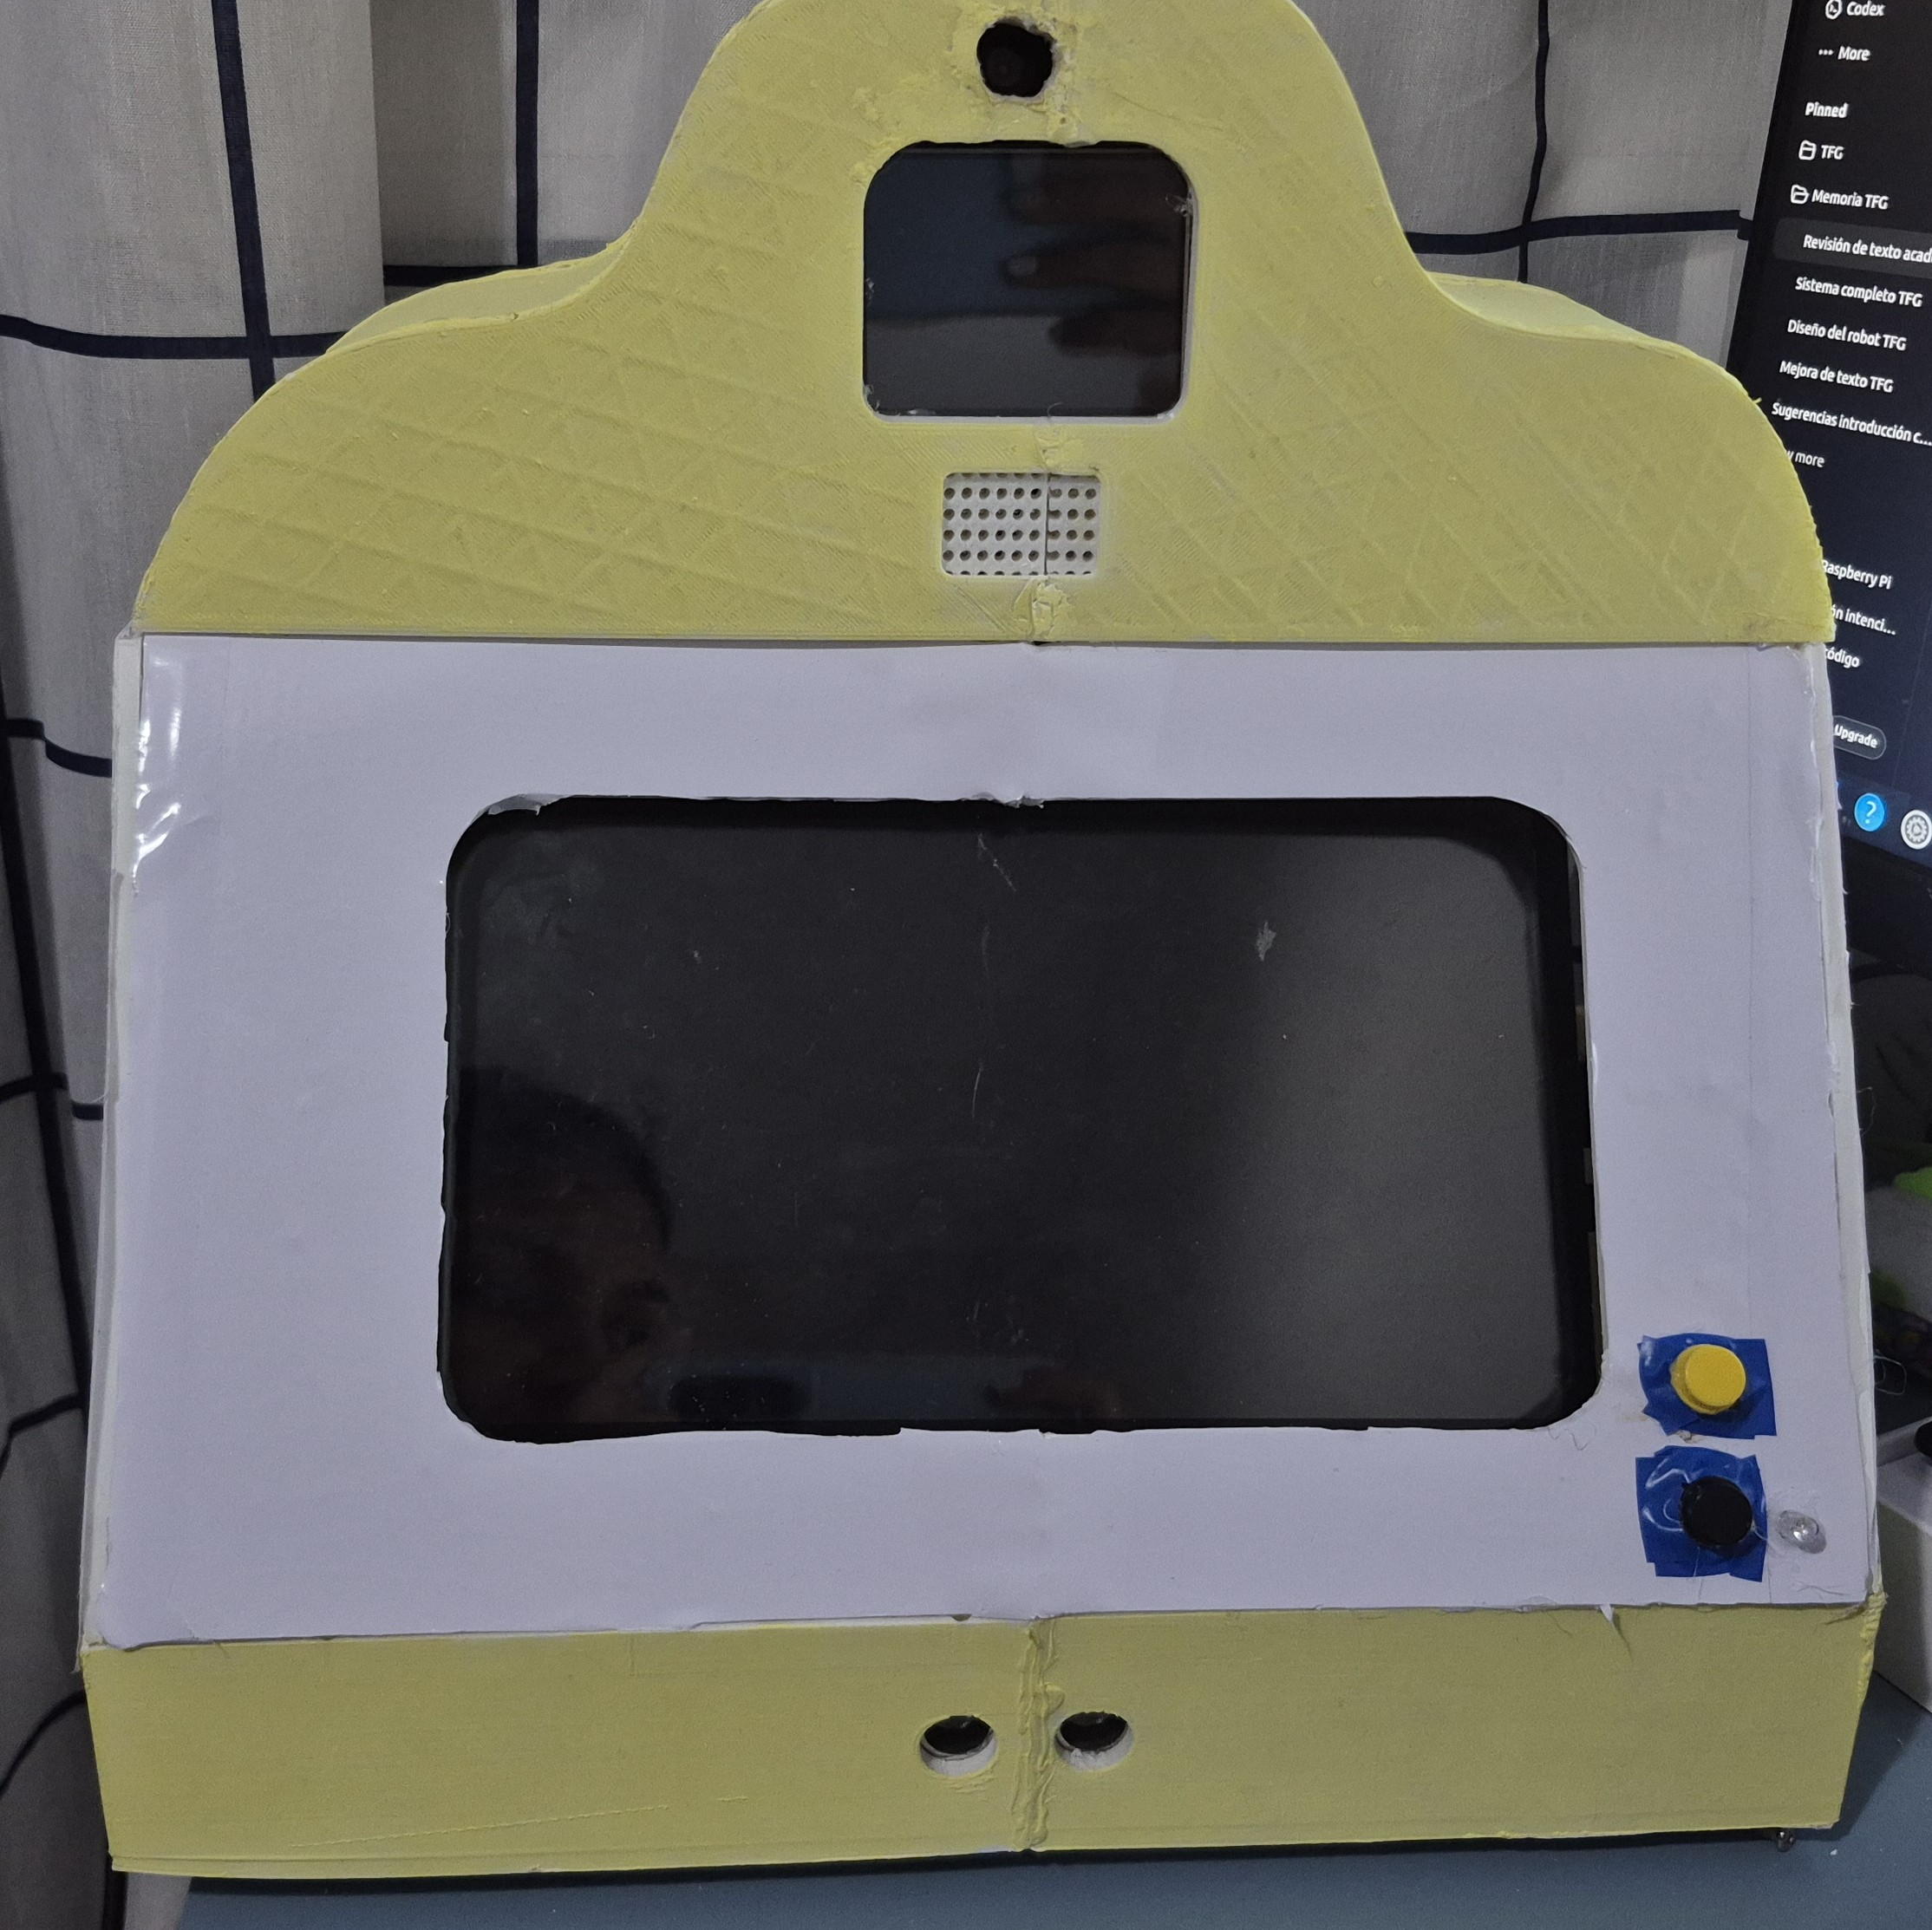
\includegraphics[width=0.48\textwidth, height=60mm, keepaspectratio=false]{figs/montaje1}}
  \end{center}
  \caption{Prototipo a cartón}
  \label{fig:robot}
\end{figure}


Tras materializar el diseño del robot, se procedió a la integración de la arquitectura electrónica, encargada de dotar al sistema de capacidades de control, sensorización e interacción.

\vspace{0.2cm}

Con el objetivo de disponer de una estructura clara, se dividió en bloques funcionales según su finalidad:

\begin{itemize}
    \item \textbf{Unidad de Control Central:} Compuesta por la Raspberry Pi 4, encargada del procesamiento. A este módulo se conectan los principales periféricos del sistema como la cámara y el micrófono para tareas de captura, así como un monitor portátil para la visualización de la interfaz.
    \item \textbf{Sistema de sensores:} Orientado a la obtención de la información del entorno. Incluye un sensor de ultrasonido para la detección de obstáculos, un pulsador para la activación del sistema, un LED RGB como indicador de estado y una pantalla LCD para mostrar mensajes informativos.
\end{itemize}

Para el diseño del circuito se utilizó la plataforma Cirkit Designer\footnote{https://app.cirkitdesigner.com/}, mediante la cual se generó el esquema electrónico del sistema (Figuras \ref{fig:circuito}).

\begin{figure} [h!]
  \begin{center}
    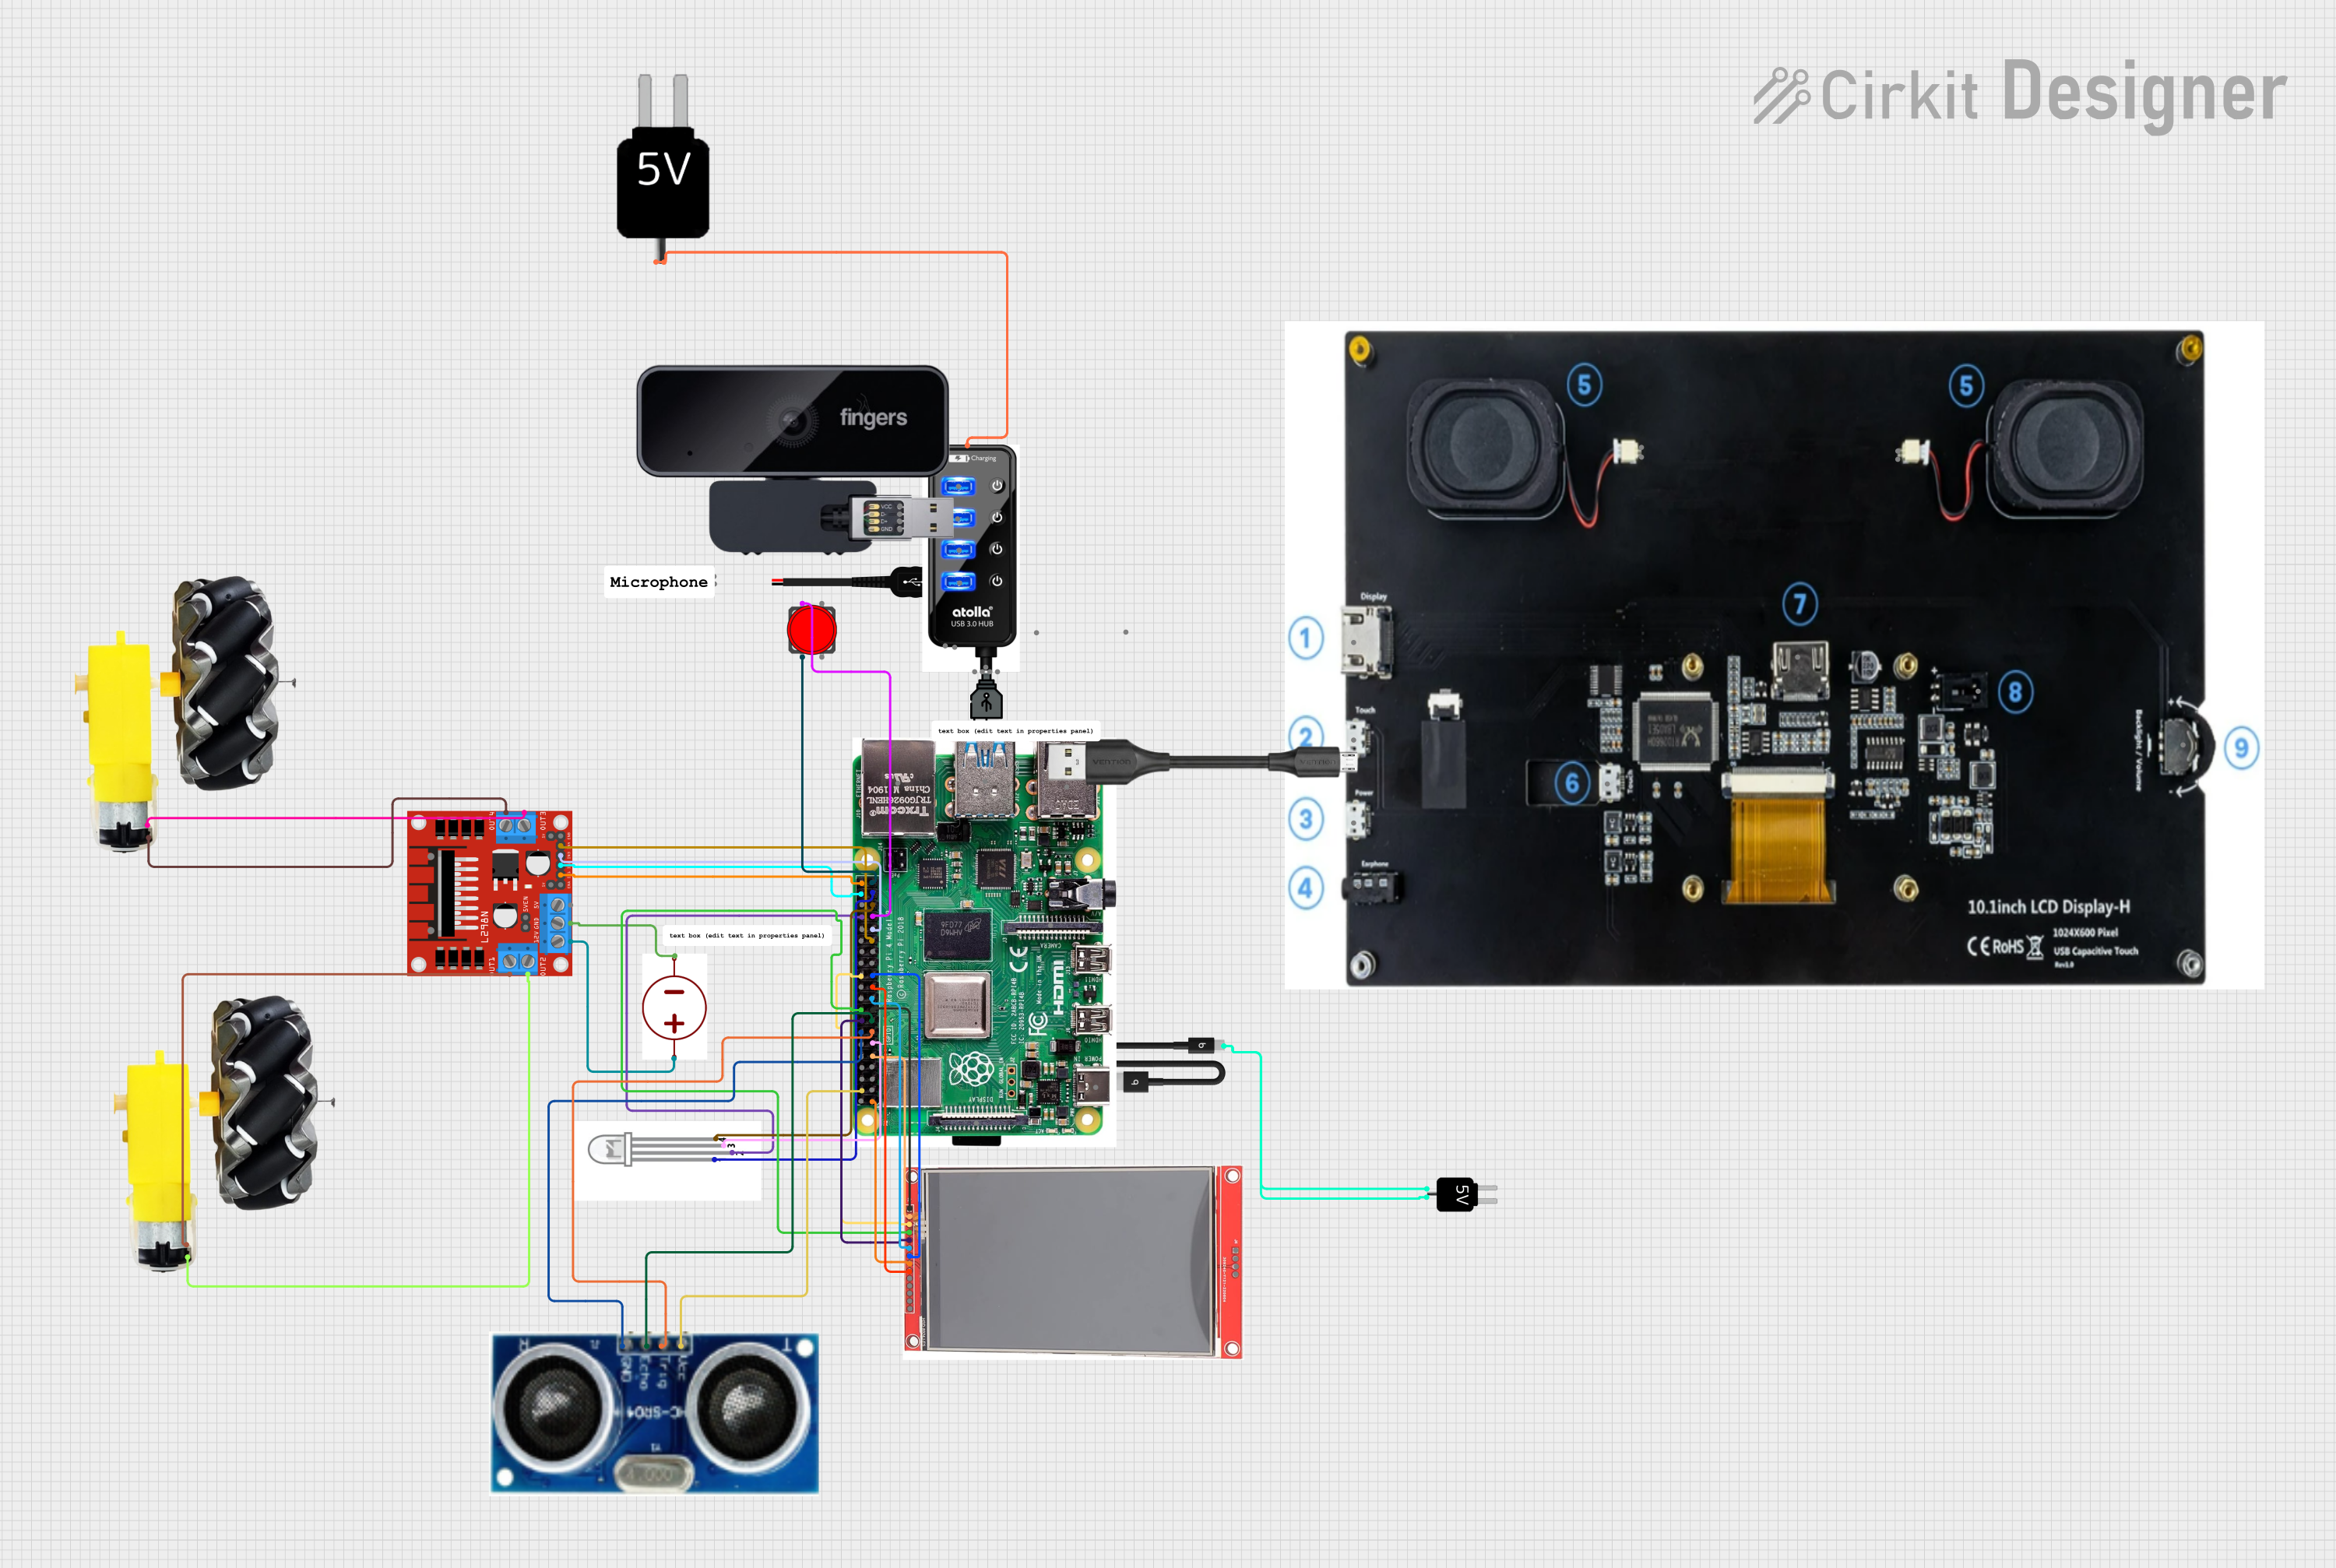
\includegraphics[width=16cm]{figs/circuit_image}
  \end{center}
  \caption{Circuito electrónico}
  \label{fig:circuito}
\end{figure}\


Con el esquema del circuito eléctrico se completa la fase de diseño e integración del  \textit{hardware} del sistema. La parte física del robot está compuesta por una estructura ligera fabricada en PLA, una base de tres ruedas que maximiza la estabilidad, y la Raspberry Pi 4 como núcleo de control.

No obstante, para que el conjunto de sensores y actuadores pueda funcionar de forma coordinada es necesaria una capa de software que permita alcanzar los objetivo de este proyecto.
